% !Mode:: "TeX:UTF-8"
% !TEX root = ..\Literature_Translation.tex
\kchapter{引言}
我们将在本文描述一个产生于飞机制造的装配夹具的生产调度问题。
我们对受邻接约束下,为了装配而用到夹具的这部分特殊飞机零件的生产特别感兴趣。夹具是用来夹紧工件或作为支撑的设备,专为适用特定零件或形状而建。
夹具的主要作用是定位,在某些情况下也用于整个加工操作中或其他工业过程的工件保持(Niu,1988;Drake,1989;Howe,2004)。
由于空间限制,夹具相邻的工作站不能同时开工,产生了邻接约束。
装配一个飞机零件至少需要2个步骤,其中之一需要在夹具上完成,另一个互补的装配操作将在工作台上进行。根据装配所需的零件,这两个操作需要重复操作。

在这项研究中,这些操作的调度考虑一个面向飞机制造的相关且实用的问题:新飞机模型的零件的组装过程的发展。总所周知,自从Wright(1936)的研究引入了飞机工业的学习曲线起,如同不同的作者所指出的,飞机装配的重复生产将会导致不同的成本和预计时间。
本文我们也对员工对特定飞机零件的装配学习或熟练进程带来的影响感兴趣。
这个装配学习进程可以分为4个主要阶段(时期),其中第1阶段是有关原型的开发和工艺过程的制定,其他3个阶段飞机已处在连续生产过程,所不同的仅为执行装配作业的队伍的能力。

研究航空工厂的装配夹具调短问题相对稀少,就我们所知,尚无其他论文在研究有关邻接约束的装配问题。
Heike, Ramulu, Sorenson, Shanahan 和Moinzadeh(2001)已分析过航空工业的结构化装配调度问题,也可以找到 Dale(2001), Chikong, Chang, Lin(2006), Abuabara 和Morabito(2009)有关航空工业的运筹学方法示例。
然而,他们都没有考虑装配夹具调度问题。该问题的预备研究可见 Silva, Morabito和 Yanasse(2011)的论文,他们给第1阶段建立了基于作业车间调度的数学模型, Silva, Morabito, Yamashita,和 Produção(2013)研究了基于项目调度的模型。这些研究都可以看作是本文研究的一些拓展。

除了航空工业,其他领域也有邻接约束的调度问题。 Santos, Michelon, Arenales,和 Santos(2008)研究了轮作调度问题,提出了一个列产生过程和一个建设性的贪心算法以解决此问题。
Weintraub等(2007)考虑了相邻区域的收获限制,提出了混合整数线性模型以对付森林砍伐调度问题。
Gandham, Dawande,和Prakash(2008)研究了由于电信网络存在的隐藏节点而导致的邻接约束问题,并通过算法求解了此问题。
Duin和 Van der Sluis(2006)研究了在机场乘客检票过程的服务台分配中,相邻资源调度的复杂性问题。
Irani和 Leung(1996,2003)在交通信号灯的调度问题中,使用基于图论的算法来研究邻接约束。
这些问题的求解方法是他们为自己量身定做的,因此,不能直接应用于本文的研究。

在先前的工作中,我们对这个特定飞机零件问题提出了不同的数学模型。
在飞机零件的装配模型中,我们考虑了员工的学习或熟练效应,他们被应用并通过GAMS 建模语言(Brooke, Kendrickd,和 Rosenthal,1998)和最优化软件CPLEX(ILOG,2011)求解。
为了验证该模型,我们通过来自巴西飞机制造商的实际数据来进行计算测验。
全文如是安排:第2节回顾文献,第3节将为各生产阶段建立数学模型,第4节呈现计算结果,第5节分析结果并展望未来研究。

\kchapter{问题描述}
为了说明,我们举例一个8零件组成的子集(装配部件),并且每一个零件都有各自相应在装配夹具的工作站。每个零件以标号1 -- 8来区分,按照总装子集的装配顺序排列。由于每架飞机的装配需要由两套完整的子集,这8类零件每个至少需要2个零件,如\reff{fig:subsetandparts}所示。
\begin{figure}[h]
\centering\caption{子集和其代表零件\label{fig:subsetandparts}}
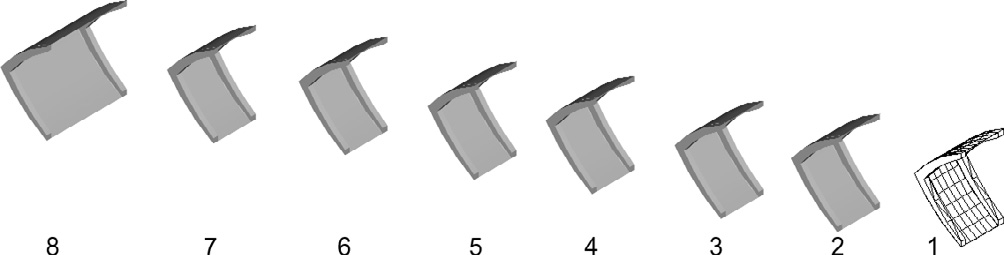
\includegraphics[width = 10cm]{Subsetanditsrespectiveparts.jpg}
\end{figure}

该子集的装配夹具有8个工作站,编号为1 -- 8,以表示与之对应的零件在此装配。
